% ===========================================================================
%  BMT317 - Algoritmalar | Proje Raporu
%  Sıralama Algoritmalarının Performans Karşılaştırması
%
%  Derleme: ./compile.sh  (assets/report dizininden)
% ===========================================================================
\documentclass[12pt,a4paper]{article}

\usepackage[T1]{fontenc}
\usepackage[utf8]{inputenc}
\usepackage{lmodern}
\usepackage[top=3cm,bottom=3cm,left=2.8cm,right=2.8cm]{geometry}
\usepackage{setspace}
\usepackage{graphicx}
\usepackage{booktabs}
\usepackage{array}
\usepackage{float}
\usepackage{caption}
\usepackage{enumitem}
\usepackage{microtype}
\usepackage{amsmath}
\usepackage{fancyhdr}
\usepackage[hidelinks,bookmarks=false,plainpages=false]{hyperref}

\newcommand{\OgrenciAdi}{Murat Yalçın}
\newcommand{\OgrenciNumarasi}{24181616002}
\newcommand{\TeslimTarihi}{29/10/2026}

% ---------------------------------------------------------------------------
% Başlıklar
% ---------------------------------------------------------------------------
\renewcommand{\contentsname}{İçindekiler}
\renewcommand{\listfigurename}{Şekiller Listesi}
\renewcommand{\listtablename}{Tablolar Listesi}
\renewcommand{\figurename}{Şekil}
\renewcommand{\tablename}{Tablo}
\renewcommand{\refname}{Kaynakça}

\setstretch{1.15}
\setlength{\parindent}{1.25cm}
\setlength{\parskip}{0.15em}
\tolerance=1000
\emergencystretch=2em
\captionsetup{font=small,labelfont=bf,skip=6pt}
\setlist[itemize]{itemsep=2pt,topsep=4pt,leftmargin=1.4em}
\setlist[enumerate]{itemsep=2pt,topsep=4pt,leftmargin=1.6em}

\pagestyle{fancy}
\fancyhf{}
\setlength{\headheight}{14pt}
\fancyhead[L]{\footnotesize BMT317 -- Algoritmalar}
\fancyhead[R]{\footnotesize Sıralama Algoritmalarının Performansı}
\fancyfoot[C]{\thepage}
\renewcommand{\headrulewidth}{0.4pt}

\begin{document}

% ===========================================================================
% KAPAK
% ===========================================================================
\hypersetup{pageanchor=false}
\begin{titlepage}
  \centering
  \thispagestyle{empty}

  \vspace*{1.2cm}
  {\Large\bfseries GAZİ ÜNİVERSİTESİ\par}
  \vspace{0.35cm}
  {\large TEKNOLOJİ FAKÜLTESİ\par}
  {\large BİLGİSAYAR MÜHENDİSLİĞİ BÖLÜMÜ\par}

  \vspace{2.4cm}
  {\large BMT317 -- ALGORİTMALAR\par}
  \vspace{0.25cm}
  {\large PROJE ÖDEVİ\par}

  \vspace{1.8cm}
  {\LARGE\bfseries Sıralama Algoritmalarının\\[0.25cm]
   Performans Karşılaştırması\par}

  \vspace{2.6cm}
  \begin{tabular}{rl}
    \textbf{Öğrenci Adı Soyadı:} & \OgrenciAdi \\[0.35cm]
    \textbf{Öğrenci Numarası:}   & \OgrenciNumarasi \\[0.35cm]
    \textbf{Tarih:}              & \TeslimTarihi \\
  \end{tabular}

  \vfill
  {\large Öğretim Elemanı: Doç. Dr. Adem Tekerek\par}
  \vspace{0.6cm}
\end{titlepage}
\hypersetup{pageanchor=true}

% ===========================================================================
% ÖZET
% ===========================================================================
\pagenumbering{roman}
\setcounter{page}{1}

\section*{Özet}
\addcontentsline{toc}{section}{Özet}

Bu rapor, yedi karşılaştırmalı sıralama algoritmasının C++17 ile
gerçekleştirilmesini ve deneysel performans karşılaştırmasını sunmaktadır.
Selection, Insertion, Bubble, Shell, Quick, Merge ve Heap Sort algoritmaları;
rastgele, sıralı, ters sıralı ve kısmen sıralı olmak üzere dört veri dağılımı ve
100 ile 100000 arasında değişen altı veri boyutu üzerinde incelenmiştir. Her
algoritma aynı başlangıç verisinin bağımsız bir kopyası üzerinde, beş ölçüm
yinelemesi ve bir ısınma turu ile çalıştırılmış; çalışma süresi, karşılaştırma
sayısı, veri hareketi sayısı ve yardımcı bellek gereksinimi kaydedilmiştir.
Sonuçlar, ikinci dereceden karmaşıklığa sahip algoritmaların büyük veri
kümelerinde $n \log n$ algoritmalara göre yaklaşık üç mertebe daha yavaş
kaldığını göstermektedir. Rastgele 100000 elemanlı veride Quick Sort 11.15 ms,
Merge Sort 12.48 ms ve Heap Sort 15.40 ms çalışırken Bubble Sort 18.23 s'ye
ulaşmıştır. Sıralı veride Insertion ve Bubble Sort doğrusal davranış sergilemiş;
log--log regresyonla elde edilen büyüme üsleri ikinci dereceden algoritmalar için
$b \approx 2$, $n \log n$ algoritmalar için $b \approx 1.1$--$1.2$ olarak
bulunmuştur. Rapor, algoritmaların güçlü ve zayıf yönlerini veri dağılımı,
bellek erişimi ve sabit maliyetler bağlamında tartışmakta ve pratik seçim
önerileri sunmaktadır.

\paragraph{}Ödevin gerçekleştirilmesinde yer alan bazı konular için yapay zeka araçlarından yardım alınmıştır.
Bu konular, rapor şablonunun \LaTeX{} formatında oluşturulması, Uygulamanın kullanılabilir bir CLI aracı
haline getirilmesi ve elde edilen verilerin grafiğe dökülmesi olarak sıralanabilir.
Ders kapsamında öğrenilen sıralama algoritmaları bu uygulamaya elle eklenmiştir.
Bunun yanı sıra ödevde beklenilen şekilde dataset oluşturulması ve kullanımı da yapay zeka aracı kullanmadan gerçekleştirilmiştir.
Raporun içeriği de elle yazılmış olup, biçimlendirilmesi, grafiklerin ve tabloların eklenmesi için yapay zekadan yardım alınmıştır.

\newpage
\tableofcontents
\newpage
\listoffigures
\newpage
\listoftables
\newpage

\pagenumbering{arabic}

% ===========================================================================
\section{Giriş}
% ===========================================================================

\paragraph{}Bu rapor kapsamında yedi algoritma ortak bir C++17 arayüzü üzerinde gerçekleştirilmiş;
rastgele, sıralı, ters sıralı ve kısmen sıralı dört veri dağılımı ile 100,
1000, 5000, 10000, 50000 ve 100000 elemanlı veri kümeleri kullanılmıştır.
Her deney beş kez yinelenmiş ve ilk çalıştırmanın başlangıç maliyetlerini elemek
için bir ısınma turu yapılmıştır. Ölçüt olarak çalışma süresi, karşılaştırma
sayısı, veri hareketi sayısı ve yardımcı bellek gereksinimi ele alınmıştır.

\paragraph{}Sonuçlar, algoritmaların kuramsal karmaşıklıklarıyla karşılaştırılmış ve
log--log regresyon ile ampirik büyüme üsleri hesaplanmıştır.

\paragraph{}Raporun izleyen bölümleri şu şekilde düzenlenmiştir: Bölüm~2'de algoritmaların
teorik temelleri ve karmaşıklıkları, Bölüm~3'te C++ gerçekleştiriminin tasarımı
ve ölçüm altyapısı, Bölüm~4'te deneysel yöntem ve ölçüm ortamı, Bölüm~5'te
deneysel bulgular, Bölüm~6'da bulguların tartışılması, Bölüm~7'de ise sonuç ve
öneriler yer almaktadır.

% ===========================================================================
\section{Teorik Bilgi}
% ===========================================================================

\subsection{Temel kavramlar}

Karşılaştırmaya dayalı sıralama algoritmaları, elemanları birbirleriyle
karşılaştırarak doğru sırayı belirler. Bu sınıfta yer alan ve yalnızca ikili
karşılaştırma kullanan hiçbir algoritma, en kötü durumda $\Omega(n \log n)$
sınırından daha hızlı olamaz. İkinci dereceden algoritmaların büyük veri
kümelerinde neden dezavantajlı hale geldiği bu alt sınırla doğrudan ilişkilidir.

Bir algoritmanın değerlendirilmesinde kullanılan başlıca kavramlar şunlardır:

\begin{itemize}
  \item \textbf{Yerinde çalışma (in-place):} Algoritmanın girdi dizisinin dışında
        yalnızca sabit miktarda ek bellek kullanmasıdır.
  \item \textbf{Kararlılık (stability):} Eşit anahtara sahip elemanların
        sıralama sonrasında başlangıçtaki göreli sıralarını korumasıdır.
  \item \textbf{Karşılaştırma sayısı:} Elemanlar arasında yapılan ikili
        karşılaştırmaların sayısıdır.
  \item \textbf{Veri hareketi:} Elemanların dizi içinde atanması, kaydırılması
        veya yer değiştirmesiyle oluşan veri taşıma işlemlerinin sayısıdır.
  \item \textbf{Yardımcı bellek:} Girdi dizisine ek olarak kullanılan bellektir;
        özyinelemeli algoritmalarda çağrı yığını da bu kapsama girer.
\end{itemize}

Bu ölçütler, yalnızca asimptotik karmaşıklığı değil, aynı zamanda sabit
maliyetleri ve bellek erişim düzenini de görünür kılar. Örneğin aynı $O(n \log n)$
sınıfında yer alan iki algoritma, önbellek dostu erişim düzeni nedeniyle belirgin
biçimde farklı sürelerde çalışabilir.

\subsection{İkinci dereceden karmaşıklığa sahip algoritmalar}

\paragraph{Selection Sort (Seçmeli Sıralama).}
Algoritma, dizinin sıralanmamış kısmındaki en küçük elemanı bulur ve onu
sıralanmamış kısmın başına taşır. Bu işlem her adımda tek bir yer değiştirme
gerektirdiğinden veri hareketi sayısı $O(n)$ düzeyinde kalır; ancak en küçük
elemanı bulmak için her durumda $n(n-1)/2$ karşılaştırma yapılır. Bu nedenle en
iyi, ortalama ve en kötü durum karmaşıklığı $O(n^2)$'dir. Algoritma yerinde
çalışır ve kararlı değildir; uzak elemanların yer değiştirmesi eşit anahtarların
göreli sırasını bozabilir.

\paragraph{Insertion Sort (Eklemeli Sıralama).}
Dizinin sol tarafında sıralı bir önek büyütülür; her yeni eleman, sıralı önek
içinde doğru konuma yerleştirilir. Elemanlar kaydırılarak yerleştirildiğinde
yalnızca bir atama ile çok sayıda eleman bir sağa kaydırılabilir. Sıralı girdide
her eleman için tek bir karşılaştırma yeterlidir; dolayısıyla en iyi durum
$O(n)$'dir. Ters sıralı girdide ise her eleman başa kadar kaydırılır ve karmaşıklık
$O(n^2)$ olur. Algoritma kararlıdır ve $O(1)$ yardımcı bellek kullanır. Küçük ve
kısmen sıralı veri kümelerinde pratikte sıkça tercih edilir.

\paragraph{Bubble Sort (Kabarcık Sıralama).}
Komşu elemanlar karşılaştırılır ve yanlış sıradaysa yer değiştirilir; her geçişte
en büyük eleman dizinin sonuna “kabarcık” gibi taşınır. Erken çıkış optimizasyonu
kullanıldığında, hiç yer değiştirmenin olmadığı bir geçişte algoritma durur ve
sıralı girdide $O(n)$ sürede tamamlanır. Ortalama ve en kötü durum karmaşıklığı
$O(n^2)$'dir. Kararlıdır ve yerinde çalışır; ancak her yer değiştirme üç veri
hareketi ürettiğinden, özellikle ters sıralı girdide veri hareketi sayısı çok
yüksektir.

\subsection{Shell Sort}

Shell Sort, Insertion Sort'un azalan artışlarla (gap) genelleştirilmiş halidir. Dizi önce belirli bir $h$ aralığındaki elemanlar kendi
aralarında sıralanır ($h$-sıralı hale getirilir), sonra $h$ küçültülür ve son adımda $h=1$
ile normal Insertion Sort uygulanır. Bu ön sıralama, son adımdaki kaydırma
sayısını önemli ölçüde azaltır.

Bu projede $n/2, n/4, \dots, 1$ biçimindeki klasik Shell gap dizisi
kullanılmıştır. Karmaşıklık kullanılan gap dizisine bağlıdır; bu dizide en kötü
durum $O(n^2)$ olabilmekle birlikte pratikte ikinci dereceden algoritmalardan
belirgin biçimde hızlıdır. Shell Sort yerinde çalışır ve kararlı değildir. Daha
iyi gap dizileri (örneğin Knuth'un $1, 4, 13, 40, \dots$ dizisi veya Ciura
dizisi) karşılaştırma sayısını daha da düşürebilir; ancak bu çalışmada tek bir
dizinin sabit tutulması, algoritmalar arası karşılaştırmanın yorumlanmasını
kolaylaştırmıştır.

\subsection{$O(n \log n)$ algoritmalar}

\paragraph{Quick Sort (Hızlı Sıralama).}
Quick Sort, bir pivot seçip diziyi pivotdan küçük ve büyük elemanlar olmak üzere
ikiye böler; ardından alt dizileri özyinelemeli olarak sıralar.
Ortalama durumda $O(n \log n)$, en kötü durumda ise bölümlemenin dengesiz
olmasına bağlı olarak $O(n^2)$ karmaşıklığa sahiptir. Pivot seçimi bu nedenle
kritiktir. Bu projede üçün ortancası (median-of-three) yöntemi kullanılmıştır.
Bu yöntem kapsamında birinci, orta ve son elemanlardan ortanca olanı pivot yapılmıştır.
Bu sayede, sıralı ve ters sıralı girdilerde dengeli bölümleme olasılığı artar.

Quick Sort yerinde çalışır ve kararlı değildir. Özyineleme yalnızca küçük
bölüm üzerinde yapılıp büyük bölüm döngüyle işlendiğinde yığın derinliği
$O(\log n)$ ile sınırlanır. Bölümleme sırasında yapılan yer değiştirmeler
bitişik olmayan bellek erişimlerine yol açsa da, küçük sabitleri ve iyi önbellek
davranışı nedeniyle pratikte çoğu zaman en hızlı genel amaçlı sıralama
algoritmalarından biridir.

\paragraph{Merge Sort (Birleştirmeli Sıralama).}
Dizi ikiye bölünür, her parça ayrı ayrı sıralanır ve iki sıralı parça tek bir
geçişte birleştirilir. Birleştirme işlemi sıralı iki listenin başlarındaki
elemanları karşılaştırarak ilerler; bu nedenle toplam karmaşıklık her durumda
$O(n \log n)$'dir. Algoritma kararlıdır; eşit elemanlarda sol parçadan gelen
eleman tercih edilir. Ancak birleştirme için $O(n)$ boyutunda yardımcı dizi
gerekir. Sıralı erişim düzeni sayesinde büyük veri kümelerinde öngörülebilir bir
performans sunar.

\paragraph{Heap Sort (Yığın Sıralama).}
Dizi bir maksimum yığın (max-heap) olarak düzenlenir; kökteki en büyük eleman
dizinin sonuna taşınır ve kalan bölüm yeniden yığın özelliğine getirilir.
Yığın kurulumu $O(n)$, her elemanın çıkarılması ise $O(\log n)$
olduğundan toplam karmaşıklık $O(n \log n)$'dir. Algoritma yerinde çalışır ve
$O(1)$ yardımcı bellek kullanır; ancak kararlı değildir. Alt dizinlere bölme 
işlemleri nedeniyle bellek erişimi Merge Sort'a göre daha dağınıktır, bu durum
özellikle büyük dizilerde önbellek başarımını olumsuz etkileyebilir.

\subsection{Karmaşıklık özeti}

Tablo~\ref{tab:teori}, yedi algoritmanın en iyi, ortalama ve en kötü durum zaman
karmaşıklıklarını; kararlılık ve yardımcı bellek özelliklerini özetlemektedir.
Buradaki değerler kuramsal sınırlardır; gerçek süreler sabit maliyetler, veri
dağılımı ve donanım özelliklerine göre değişir.

\begin{table}[htbp]
  \centering
  \caption{Yedi algoritmanın kuramsal zaman karmaşıklıkları, kararlılık ve
           yardımcı bellek özellikleri.}
  \label{tab:teori}
  \small
  \begin{tabular}{lcccc l}
    \toprule
    Algoritma & En iyi & Ortalama & En kötü & Kararlı & Yardımcı bellek \\
    \midrule
    Selection Sort & $O(n^2)$ & $O(n^2)$ & $O(n^2)$ & Hayır & $O(1)$ \\
    Insertion Sort & $O(n)$   & $O(n^2)$ & $O(n^2)$ & Evet  & $O(1)$ \\
    Bubble Sort    & $O(n)$   & $O(n^2)$ & $O(n^2)$ & Evet  & $O(1)$ \\
    Shell Sort     & Değişken & Değişken & $O(n^2)$ & Hayır & $O(1)$ \\
    Quick Sort     & $O(n \log n)$ & $O(n \log n)$ & $O(n^2)$ & Hayır & $O(\log n)$ \\
    Merge Sort     & $O(n \log n)$ & $O(n \log n)$ & $O(n \log n)$ & Evet & $O(n)$ \\
    Heap Sort      & $O(n \log n)$ & $O(n \log n)$ & $O(n \log n)$ & Hayır & $O(1)$ \\
    \bottomrule
  \end{tabular}

  \par\smallskip
  \footnotesize Shell Sort'un karmaşıklığı kullanılan gap dizisine bağlıdır; bu
  projede $n/2, n/4, \dots, 1$ dizisi kullanılmıştır. Quick Sort'un $O(\log n)$
  yardımcı belleği, yalnızca küçük bölüm üzerinde özyineleme yapıldığında
  geçerlidir.
\end{table}

% ===========================================================================
\section{Algoritmaların Gerçekleştirilmesi}
% ===========================================================================

\subsection{Dil, araçlar ve genel yapı}

Proje C++17 standardı kullanılarak geliştirilmiştir. Derleme
sistemi olarak Meson ve Ninja kullanılmış; kod, Windows (MSVC veya MinGW) ve
POSIX sistemlerde aynı kaynaklardan derlenebilecek şekilde taşınabilir
tutulmuştur. İşletim sistemine özgü başlık veya çağrı kullanılmamıştır. Süre
ölçümünde \texttt{std::chrono::steady\_clock} tercih edilmiştir. 

Proje kaynak kodu işlevsel olarak ayrılmıştır:

\begin{itemize}
  \item \texttt{src/core}: eleman tipi, ölçüm sayaçları, veri üretimi,
        \texttt{is\_sorted()} kontrolü ve kronometre.
  \item \texttt{src/algorithms}: her algoritma için ayrı bir derleme birimi ve
        algoritmaları ortak bir tanımlayıcıyla sunan kayıt (registry) yapısı.
  \item \texttt{src/bench}: deney planı, veri kopyalama, ısınma turları,
        yinelemeler ve sonuçların toplanması.
  \item \texttt{src/cli} ve \texttt{src/io}: komut satırı ayrıştırma ve CSV
        yazımı.
  \item \texttt{tests}: algoritmaların doğruluğunu, sayaçları, ayrıştırıcıyı ve
        uçtan uca bir deneyi sınayan testler.
\end{itemize}

Projenin kaynak koduna
\url{https://github.com/muratyalcin-ce/sortbench} adresinden erişilebilir.

Projede hazır sıralama fonksiyonları kullanılmamıştır. Bütün sıralama
fonksiyonları elle implemente edilmiştir.

\subsection{Ortak ölçüm altyapısı}

Tüm algoritmalar aynı arayüzü kullanır:

\begin{verbatim}
using Value = std::int32_t;
using SortFn = void (*)(std::vector<Value>&, SortContext&);
\end{verbatim}

\texttt{SortContext}, algoritmaya ölçüm sayaçlarını, önceden boyutlandırılmış
bir yardımcı tamponu ve ileride rastgele pivot gibi varyantlar için
kullanılabilecek bir rastgele sayı durumunu taşır. Yardımcı tampon, süre ölçümü
başlamadan önce ayrılır, bellek ayırma maliyeti ölçülen süreye karışmaz.
Yalnızca Merge Sort bu tamponu kullanır, diğer algoritmalar yerinde çalışır.

Karşılaştırma ve veri hareketi sayıları algoritmaların içinde, \texttt{Metrics}
yapısı üzerinden artırılır. Bu raporda kullanılan tanımlar şunlardır:

\begin{itemize}
  \item \textbf{Karşılaştırma:} İki eleman arasında yapılan her ikili
        karşılaştırma bir kez sayılır. Ölçüm yardımcıları
        (\texttt{less}, \texttt{less\_equal}) bu sayacı otomatik artırır.
  \item \textbf{Veri hareketi:} Diziye yapılan her eleman ataması bir hareket
        sayılır. Bir yer değiştirme (swap) klasik analizle uyumlu olarak üç
        hareket kabul edilir: geçici değişkene alma, birinci atama ve ikinci
        atama.
\end{itemize}

Bu tanımlar, farklı algoritmaların aynı ölçütle karşılaştırılabilmesini sağlar.
Sayaçlar örnekleme yoluyla değil, algoritmanın her karşılaştırma ve atama
noktasında doğrudan artırılır, bu nedenle aynı girdi için deterministik
algoritmalarda yinelemeler arasında birebir aynı değerler elde edilir.

\subsection{Algoritmaların gerçekleştirim ayrıntıları}

\paragraph{Selection Sort.} Sıralanmamış bölümdeki en küçük elemanın indisi
tutulur; yalnızca gerektiğinde yer değiştirme yapılır. Karşılaştırma sayısı
girdiden bağımsız olarak her zaman $n(n-1)/2$'dir, bu özellik sayaç
doğrulamasında referans olarak kullanılmıştır.

\paragraph{Insertion Sort.} Anahtar bir geçici değişkende tutulur, büyük
elemanlar bir sağa kaydırılır ve anahtar boşalan konuma yazılır. Kaydırma
sırasında yalnızca gerçekten yapılan atamalar sayılır; anahtarın yerinde kaldığı
durumlarda gereksiz yazma yapılmaz.

\paragraph{Bubble Sort.} Her geçişte komşu elemanlar karşılaştırılır; geçiş
sırasında hiç yer değiştirme olmazsa döngü sonlandırılır. Bu erken çıkış, sıralı
girdide tek bir $O(n)$ geçiş sağlar.

\paragraph{Shell Sort.} Gap dizisi $n/2$'den başlar ve her adımda ikiye bölünür.
Her gap için, o aralıktaki elemanlar üzerinde Insertion Sort'un kaydırmalı
varyantı uygulanır. Gap dizisi sabit tutularak deneylerin tekrarlanabilirliği
korunmuştur.

\paragraph{Quick Sort.} Pivot olarak birinci, orta ve son elemanın ortancası
seçilir; pivot son konuma taşınır ve Lomuto bölümleme şeması uygulanır. İki
elemanlı aralıklar ayrıca ele alınır çünkü bu durumda orta eleman birinci veya
son elemanla çakışır. Özyineleme yalnızca küçük alt bölüm için yapılır, büyük alt
bölüm döngüyle işlenir. Böylece en kötü durumda bile yığın derinliği $O(\log n)$
düzeyinde tutulur.

\paragraph{Merge Sort.} Yukarıdan aşağıya (top-down) bölme yaklaşımı
kullanılmıştır. Birleştirme sırasında sağ parçadan eleman alınması yalnızca
\texttt{a[j]} $<$ \texttt{a[i]} koşulu sağlandığında yapılır, eşitlik durumunda sol parça
tercih edilerek kararlılık korunur. Yardımcı dizi, bağlam nesnesindeki tek bir
tampondur ve tüm birleştirmelerde yeniden kullanılır.

\paragraph{Heap Sort.} Dizi, dizi tabanlı maksimum yığın olarak
uygulanmıştır. Önce iç düğümler üzerinde aşağı doğru eleme (heapify/sift-down) yapılarak
$O(n)$ sürede yığın kurulur, bunun ardından kök her adımda son elemanla değiştirilip
yığın küçültülerek sıralama tamamlanır.

\subsection{Doğruluk kontrolü ve testler}

Her ölçülen çalıştırmadan sonra sonuç, projede geliştirilen
\texttt{is\_sorted()} fonksiyonuyla kontrol edilir. Bu fonksiyon, dizinin
azalan sırada olmayan bir çift içerip içermediğini doğrusal zamanda denetler.
Ek olarak sonuç, aynı girdinin projenin kendi Merge Sort gerçekleştirimiyle
sıralanmış bir referans kopyasıyla karşılaştırılır, bu sayede sıralanma durumunun yanı sıra
dizideki verilerde oluşan hatalar da algılanır. Bir uyuşmazlık
tespit edilirse durum standart hata akışına yazılır, ilgili CSV satırı
\texttt{verified = 0} olarak işaretlenir ve program sıfır dışında bir çıkış kodu
döndürür.

Doğruluk testleri yedi algoritmayı dört dağılım ve 0, 1, 2, 3, 5, 8, 17, 64, 257
ve 1023 elemanlı veri kümeleri üzerinde referans sonuçla karşılaştırır. Ayrıca
tüm elemanları eşit ve yalnızca iki farklı değer içeren girdiler, 100 rastgele
denemeden oluşan bir fark testi (differential fuzz), sayaç beklentileri, komut
satırı ayrıştırma ve uçtan uca küçük bir deney sınanır. Test paketinde toplam
1523 kontrol bulunmakta ve tamamı başarıyla geçmektedir.

% ===========================================================================
\section{Deneysel Çalışma}
% ===========================================================================

\subsection{Ölçüm ortamı}

Deneyler tek bir makinede, diğer yoğun iş yüklerinden bağımsız olarak
gerçekleştirilmiştir. Ölçüm ortamına ilişkin bilgiler Tablo~\ref{tab:environment}
içinde verilmiştir. Süreler duvar saati (wall-clock) üzerinden ölçüldüğü için
işlemci frekansı, önbellek durumu ve arka plan etkinlikleri sonuçlara küçük de
olsa etki edebilir; bu nedenle yorumlarda mutlak sürelerden çok algoritmalar
arasındaki göreli farklar ve büyüme eğilimleri esas alınmıştır.

% Generated by scripts/analyze_results.py from results.csv.
% Do not edit by hand: regenerate with the command in assets/plots/README.md.

\begin{table}[htbp]
  \centering
  \caption{Ölçüm ortamı ve deney parametreleri.}
  \label{tab:environment}
  \footnotesize
  \begin{tabular}{@{}p{0.24\linewidth}p{0.68\linewidth}@{}}
    \toprule
    Öğe & Değer \\
    \midrule
    İşlemci & Intel(R) Core(TM) i5-1035G1 CPU @ 1.00GHz \\
    Çekirdek / iş parçacığı & 4 / 8 \\
    Bellek (RAM) & 7.6 GiB \\
    İşletim sistemi & Artix Linux \\
    Derleyici & c++ (GCC) 16.2.1 20260810 \\
    Dil standardı & C++17 \\
    Derleme sistemi & Meson 1.12.1 + Ninja (optimize ikili) \\
    IDE / çalıştırma ortamı & Komut satırı \\
    Veri boyutları & 100, 1000, 5000, 10000, 50000, 100000 \\
    Dağılımlar & rastgele, sıralı, ters sıralı, kısmen sıralı \\
    Temel tohum & 42 \\
    Yineleme & 5 ölçülmüş + 1 ısınma turu \\
    Komut & \texttt{\detokenize{sortbench --reps 5 --warmup 1}} \\
    Çalıştırma tarihi & 2026-10-24 \\
    \bottomrule
  \end{tabular}
\end{table}


\subsection{Veri kümeleri ve dağılımlar}

Deneylerde dört farklı veri dağılımı kullanılmıştır:

\begin{itemize}
  \item \textbf{Rastgele:} Elemanlar $[0, n)$ aralığında düzgün dağılımlı
        olarak üretilmiştir. Bu dağılım, algoritmanın ortalama davranışını
        yansıtır.
  \item \textbf{Sıralı:} Dizi $0, 1, \dots, n-1$ biçiminde artan sırada
        üretilmiştir.
  \item \textbf{Ters sıralı:} Dizi $n-1, \dots, 1, 0$ biçiminde azalan sırada
        üretilmiştir.
  \item \textbf{Kısmen sıralı:} Dizi artan sırada üretildikten sonra yaklaşık
        $n/10$ kez rastgele iki konumdaki eleman yer değiştirilmiştir. Böylece
        elemanların büyük bölümü sıralı kalırken yerel düzensizlikler
        oluşturulur.
\end{itemize}

Veri boyutları 100, 1000, 5000, 10000, 50000 ve 100000 olarak seçilmiştir.
Tüm veri kümeleri 64 bit Mersenne Twister (\texttt{std::mt19937\_64}) ile üretilmiştir.
Taban tohum 42'dir, her (dağılım, boyut, yineleme) üçlüsü için tohum splitmix64 ile türetilir.
Böylece deney tek bir komutla birebir yeniden üretilebilir.

\subsection{Deney protokolü}

Adil bir karşılaştırma için her yinelemede aşağıdaki sıra izlenir:

\begin{enumerate}
  \item İlgili dağılım ve boyut için temel veri kümesi bir kez üretilir.
  \item Her algoritma için temel veri kümesinin bağımsız bir kopyası alınır.
        Kopyalama, süre ölçümü başlamadan önce yapılır.
  \item Algoritma, yalnızca sıralama çağrısı kronometre içinde olacak şekilde
        çalıştırılır.
  \item Sonuç \texttt{is\_sorted()} ve referans Merge Sort karşılaştırmasıyla
        doğrulanır.
  \item Süre, karşılaştırma ve veri hareketi değerleri toplanır.
\end{enumerate}

Her deney beş kez yinelenir ve aritmetik ortalama alınır; ayrıca standart
sapma, en küçük ve en büyük süreler CSV çıktısında saklanır. İlk çalıştırmanın
sayfa hatası, önbellek ısınması ve dinamik bağlayıcı maliyetlerinden etkilenmesini
önlemek için her (algoritma, dağılım, boyut) üçlüsü için bir ısınma turu yapılır
ve bu turun sonucu hesaba katılmaz.

Ölçümlerde yalnızca sıralama fonksiyonunun kendisi kronometreye dahil edilir;
veri üretimi, kopyalama, doğrulama ve CSV yazımı süre dışındadır. Bu tercih,
algoritmaların kendi maliyetlerini öne çıkarır. Bench tarafında ayrıca
$O(n^2)$ algoritmalarının çok büyük boyutlarda uzun sürmesi durumunda deneyi
kısaltmaya yarayan bir \texttt{--quadratic-limit} seçeneği bulunur; bu rapordaki
tüm sonuçlarda sınır kullanılmamış, yedi algoritma da 100000 elemana kadar
çalıştırılmıştır.

Sonuçlar CSV biçiminde kaydedilmiş ve \texttt{assets/plots/results.csv}
dosyasında arşivlenmiştir. Her satır bir algoritma, dağılım ve boyut üçlüsü için
ortalama süre, standart sapma, en küçük/en büyük süre, ortalama karşılaştırma
sayısı, ortalama veri hareketi ve doğrulama durumunu içerir. Tablo ve şekiller bu
CSV'den \texttt{scripts/analyze\_results.py} ile üretilmiştir.

\subsection{Yeniden üretim}

Deneyler aşağıdaki komutlarla yeniden üretilebilir:

\begin{verbatim}
meson setup build --buildtype=release
meson compile -C build
meson test -C build --print-errorlogs
./build/src/sortbench --reps 5 --warmup 1 \
    --out assets/plots/results.csv
python3 scripts/analyze_results.py \
    --csv assets/plots/results.csv --outdir assets/plots
\end{verbatim}

\texttt{sortbench} programı varsayılan olarak yedi algoritma, dört dağılım ve
altı farklı veri seti boyutu çalıştırır. Seçenekler \texttt{--help}, algoritma listesi ise
\texttt{--list} ile görüntülenebilir.

% ===========================================================================
\section{Performans Sonuçları}
% ===========================================================================

Bu bölümdeki tüm süreler beş ölçümün ortalamasıdır; karşılaştırma ve veri
hareketi değerleri de aynı yinelemeler üzerinden ortalanmıştır. Ölçek farkları
nedeniyle şekillerde her iki eksen de logaritmiktir.

% Generated by scripts/analyze_results.py from results.csv.
% Do not edit by hand: regenerate with the command in assets/plots/README.md.

% Requires \usepackage{graphicx}.
% Paths assume the report is compiled from assets/report/.

\begin{figure}[htbp]
  \centering
  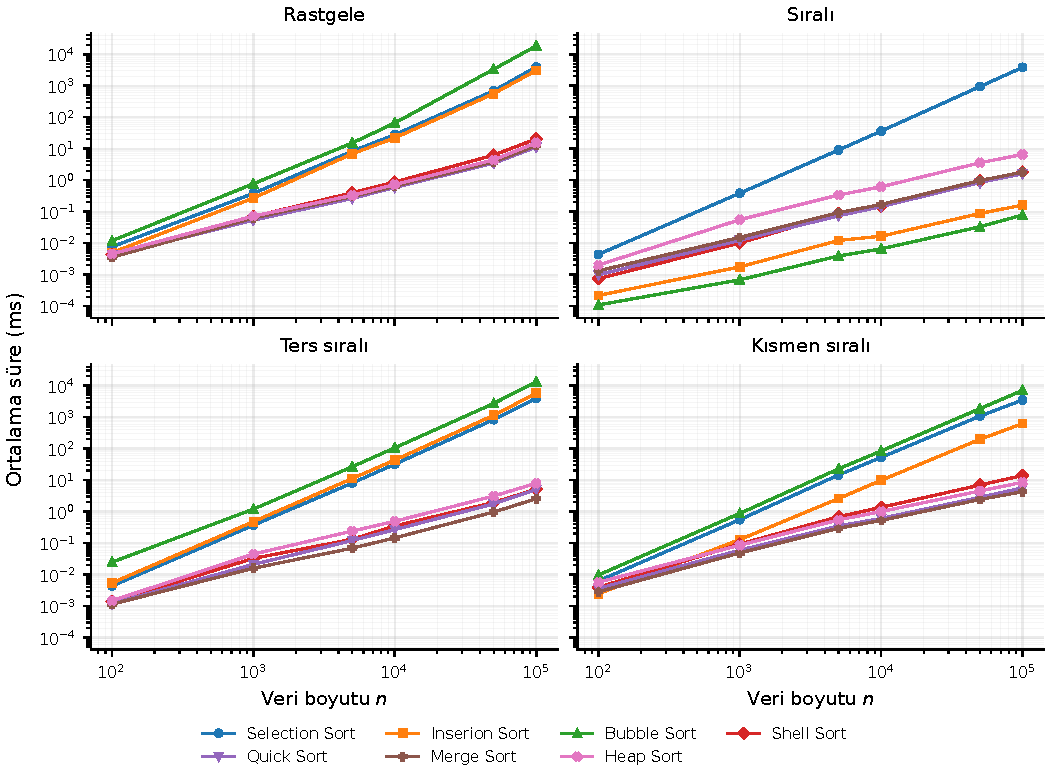
\includegraphics[width=\linewidth]{../plots/figures/fig_time_vs_n.pdf}
  \caption{Dört veri dağılımı için ortalama çalışma süresinin veri
           boyutuna göre değişimi (log--log eksenler, 5 yineleme
           ortalaması).}
  \label{fig:time}
\end{figure}

\begin{figure}[htbp]
  \centering
  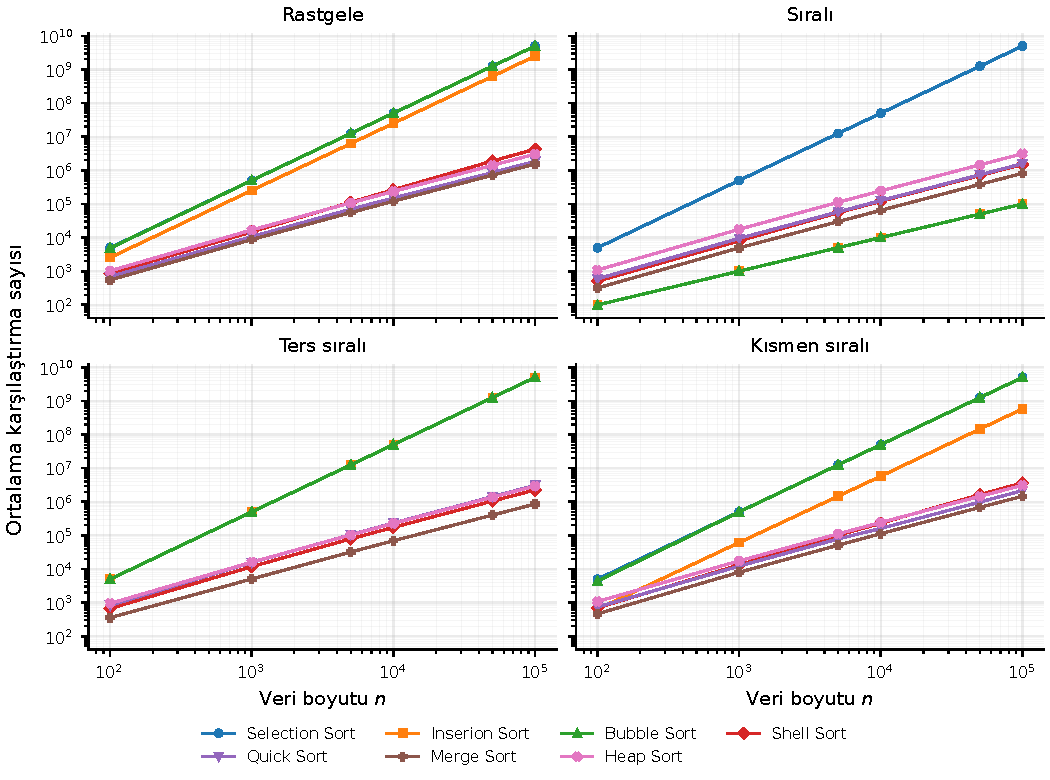
\includegraphics[width=\linewidth]{../plots/figures/fig_comparisons_vs_n.pdf}
  \caption{Ortalama karşılaştırma sayısının veri boyutuna göre değişimi
           (log--log eksenler, 5 yineleme ortalaması).}
  \label{fig:comparisons}
\end{figure}

\begin{figure}[htbp]
  \centering
  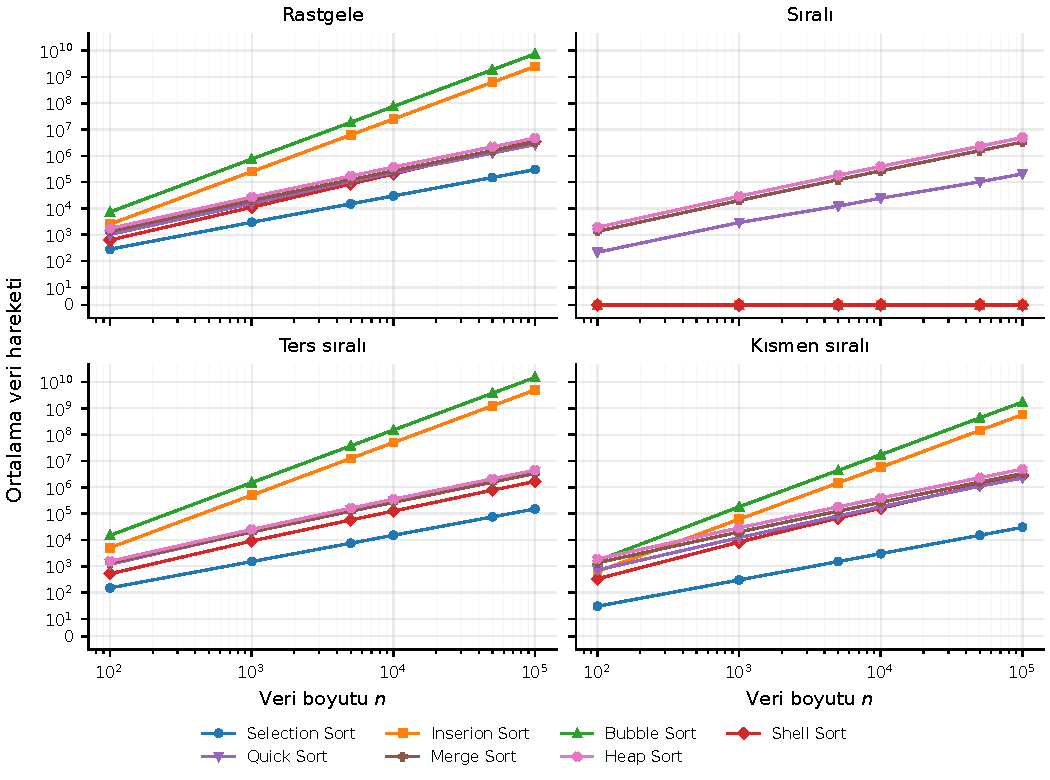
\includegraphics[width=\linewidth]{../plots/figures/fig_moves_vs_n.pdf}
  \caption{Ortalama veri hareketi sayısının veri boyutuna göre değişimi
           (5 yineleme ortalaması). Bir yer değiştirme üç hareket
           sayılmıştır; sıfır hareketli durumların görünmesi için düşey eksen
           simetrik logaritmik ölçektedir.}
  \label{fig:moves}
\end{figure}

\begin{figure}[htbp]
  \centering
  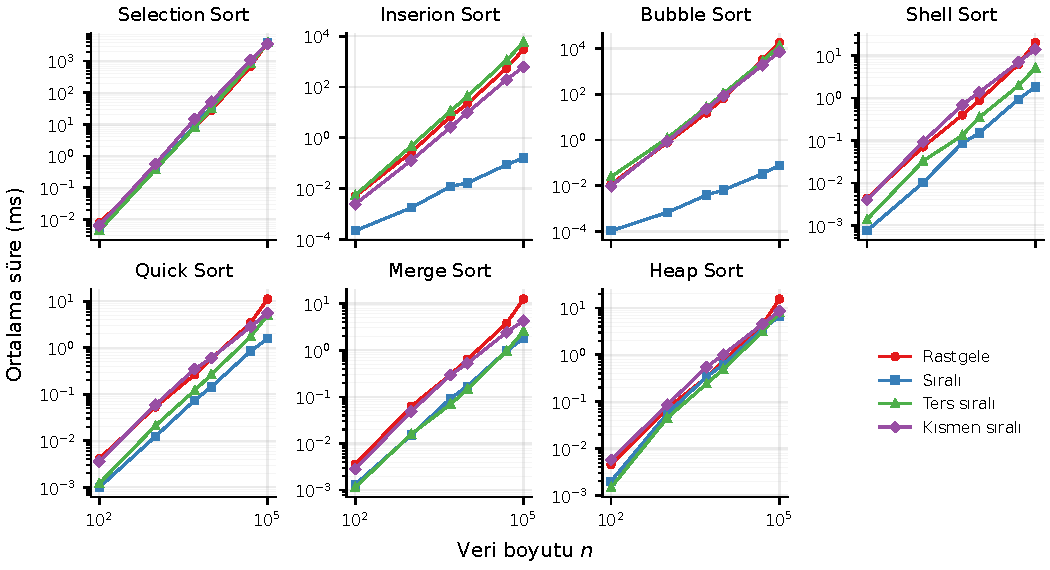
\includegraphics[width=\linewidth]{../plots/figures/fig_distribution_effect.pdf}
  \caption{Veri dağılımının çalışma süresine etkisi; her panel bir algoritma
           (log--log eksenler, 5 yineleme ortalaması).}
  \label{fig:distribution}
\end{figure}


\subsection{Çalışma süresi}

Tablo~\ref{tab:time} ve Şekil~\ref{fig:time}, çalışma süresinin veri boyutu ve
dağılımıyla değişimini göstermektedir. Rastgele veride 100000 eleman için
Selection Sort 3910 ms, Insertion Sort 3042 ms ve Bubble Sort 18233 ms
sürerken; Shell Sort 20.40 ms, Heap Sort 15.40 ms, Merge Sort 12.48 ms ve Quick
Sort 11.15 ms düzeyinde kalmıştır. Quick Sort, aynı boyuttaki Bubble Sort'tan
yaklaşık 1635 kat, Merge Sort'tan ise yaklaşık \%10 daha hızlıdır. Bu fark,
$O(n^2)$ ile $O(n \log n)$ arasındaki asimptotik ayrımın doğrudan bir
sonucudur.

% Generated by scripts/analyze_results.py from results.csv.
% Do not edit by hand: regenerate with the command in assets/plots/README.md.

\begin{table}[htbp]
  \centering
  \caption{Algoritma ve veri dağılımına göre ortalama çalışma süresi (5 yineleme ortalaması, ms).}
  \label{tab:time}
  \footnotesize
  \setlength{\tabcolsep}{3pt}
  \begin{tabular}{llrrrrrr}
    \toprule
    & \multicolumn{6}{c}{Veri boyutu $n$} \\
    \cmidrule(lr){3-8}
    Algoritma & Dağılım & $100$ & $1\,000$ & $5\,000$ & $10\,000$ & $50\,000$ & $100\,000$ \\
    \midrule
    Selection Sort & Rastgele & $0.00764$ & $0.3804$ & $8.29$ & $27.82$ & $686.6$ & $3\,910$ \\
     & Sıralı & $0.00439$ & $0.3845$ & $9.06$ & $36.18$ & $938.7$ & $3\,812$ \\
     & Ters sıralı & $0.00433$ & $0.3684$ & $8.08$ & $31.97$ & $830.5$ & $3\,899$ \\
     & Kısmen sıralı & $0.00629$ & $0.5543$ & $14.56$ & $52.57$ & $1\,077$ & $3\,495$ \\
    \midrule
    Inserion Sort & Rastgele & $0.00500$ & $0.2708$ & $6.87$ & $22.02$ & $555.6$ & $3\,042$ \\
     & Sıralı & $0.00022$ & $0.00176$ & $0.0121$ & $0.0166$ & $0.0874$ & $0.1612$ \\
     & Ters sıralı & $0.00543$ & $0.4788$ & $11.21$ & $43.34$ & $1\,137$ & $5\,714$ \\
     & Kısmen sıralı & $0.00245$ & $0.1289$ & $2.60$ & $9.84$ & $196.9$ & $621.4$ \\
    \midrule
    Bubble Sort & Rastgele & $0.0119$ & $0.7680$ & $15.16$ & $65.37$ & $3\,315$ & $18\,233$ \\
     & Sıralı & $0.00011$ & $0.00068$ & $0.00393$ & $0.00656$ & $0.0332$ & $0.0782$ \\
     & Ters sıralı & $0.0248$ & $1.20$ & $26.54$ & $105.8$ & $2\,706$ & $13\,196$ \\
     & Kısmen sıralı & $0.00968$ & $0.8742$ & $22.77$ & $83.93$ & $1\,853$ & $7\,044$ \\
    \midrule
    Shell Sort & Rastgele & $0.00430$ & $0.0702$ & $0.3977$ & $0.8741$ & $6.21$ & $20.40$ \\
     & Sıralı & $0.00074$ & $0.0102$ & $0.0870$ & $0.1484$ & $0.9332$ & $1.82$ \\
     & Ters sıralı & $0.00136$ & $0.0326$ & $0.1320$ & $0.3490$ & $1.94$ & $5.12$ \\
     & Kısmen sıralı & $0.00394$ & $0.0929$ & $0.6879$ & $1.36$ & $6.95$ & $13.97$ \\
    \midrule
    Quick Sort & Rastgele & $0.00413$ & $0.0534$ & $0.2630$ & $0.5884$ & $3.45$ & $11.15$ \\
     & Sıralı & $0.00099$ & $0.0124$ & $0.0742$ & $0.1445$ & $0.8472$ & $1.58$ \\
     & Ters sıralı & $0.00121$ & $0.0210$ & $0.1205$ & $0.2672$ & $1.75$ & $4.99$ \\
     & Kısmen sıralı & $0.00359$ & $0.0595$ & $0.3487$ & $0.6065$ & $2.85$ & $5.63$ \\
    \midrule
    Merge Sort & Rastgele & $0.00358$ & $0.0628$ & $0.3006$ & $0.6393$ & $3.80$ & $12.48$ \\
     & Sıralı & $0.00132$ & $0.0152$ & $0.0929$ & $0.1694$ & $0.9722$ & $1.79$ \\
     & Ters sıralı & $0.00114$ & $0.0159$ & $0.0690$ & $0.1462$ & $0.9649$ & $2.56$ \\
     & Kısmen sıralı & $0.00283$ & $0.0488$ & $0.2962$ & $0.5241$ & $2.43$ & $4.27$ \\
    \midrule
    Heap Sort & Rastgele & $0.00456$ & $0.0724$ & $0.3284$ & $0.7289$ & $4.39$ & $15.40$ \\
     & Sıralı & $0.00201$ & $0.0554$ & $0.3380$ & $0.6168$ & $3.56$ & $6.56$ \\
     & Ters sıralı & $0.00148$ & $0.0447$ & $0.2402$ & $0.4917$ & $3.11$ & $7.91$ \\
     & Kısmen sıralı & $0.00570$ & $0.0856$ & $0.5450$ & $1.01$ & $4.52$ & $8.52$ \\
    \bottomrule
  \end{tabular}
\end{table}


Sıralı veride tablo belirgin biçimde değişmektedir. Selection Sort, en küçük
elemanı bulmak için yine tüm karşılaştırmaları yaptığından 3812 ms'de kalır.
Buna karşılık Insertion Sort 0.161 ms, Bubble Sort 0.078 ms ile neredeyse sabit
maliyetli hale gelir; çünkü her eleman için tek karşılaştırma yeterlidir ve
kaydırma yapılmaz. Quick Sort 1.579 ms, Merge Sort 1.794 ms, Shell Sort 1.825 ms
ve Heap Sort 6.562 ms ile $O(n \log n)$ sınıfında beklenen davranışı gösterir.
Quick Sort'un sıralı veride rastgele veriden daha hızlı olması, median-of-three
pivotunun neredeyse dengeli bölümleme üretmesi ve yer değiştirme sayısının
azalmasıyla açıklanabilir.

Ters sıralı veride Insertion Sort 5714 ms ve Bubble Sort 13196 ms'ye
yükselir; her eleman başa veya sona doğru taşınır. Selection Sort 3899 ms ile
boyuttan bağımsız karşılaştırma sayısını yansıtır. Merge Sort 2.557 ms ile en
hızlı sonucu verir. Quick Sort 4.995 ms, Shell Sort 5.125 ms ve Heap Sort
7.910 ms ile izler. Kısmen sıralı veride Insertion Sort 621.4 ms olarak ölçülmüştür;
bu, az sayıda yerel düzensizliğin kaydırma maliyetini sınırlaması sayesinde
oluşur. Bubble Sort ise 7044 ms ile hâlâ yüksektir; çünkü yerel bir düzensizlik
bile çok sayıda komşu yer değiştirmeye yol açabilir.

\subsection{Karşılaştırma sayısı}

Tablo~\ref{tab:comparisons} ve Şekil~\ref{fig:comparisons}, karşılaştırma
sayılarının teorik bilgiye uyumunu göstermektedir. 100000 elemanlı
rastgele veride Selection Sort ve Bubble Sort yaklaşık $5.0 \times 10^9$,
Insertion Sort $2.5 \times 10^9$ karşılaştırma yapmıştır. Bu değerler
$n(n-1)/2$ ve $n^2/4$ mertebeleriyle uyumludur. Aynı boyutta Shell Sort
$4.24 \times 10^6$, Heap Sort $3.02 \times 10^6$, Quick Sort
$1.85 \times 10^6$ ve Merge Sort $1.54 \times 10^6$ karşılaştırma ile
$O(n \log n)$ davranışını doğrulamaktadır.

% Generated by scripts/analyze_results.py from results.csv.
% Do not edit by hand: regenerate with the command in assets/plots/README.md.

\begin{table}[htbp]
  \centering
  \caption{Algoritma ve veri dağılımına göre ortalama karşılaştırma sayısı (5 yineleme ortalaması). $10^5$ ve üzeri değerler bilimsel gösterimle verilmiştir.}
  \label{tab:comparisons}
  \footnotesize
  \setlength{\tabcolsep}{3pt}
  \begin{tabular}{llrrrrrr}
    \toprule
    & \multicolumn{6}{c}{Veri boyutu $n$} \\
    \cmidrule(lr){3-8}
    Algoritma & Dağılım & $100$ & $1\,000$ & $5\,000$ & $10\,000$ & $50\,000$ & $100\,000$ \\
    \midrule
    Selection Sort & Rastgele & $4\,950$ & $5.00\times10^{5}$ & $1.25\times10^{7}$ & $5.00\times10^{7}$ & $1.25\times10^{9}$ & $5.00\times10^{9}$ \\
     & Sıralı & $4\,950$ & $5.00\times10^{5}$ & $1.25\times10^{7}$ & $5.00\times10^{7}$ & $1.25\times10^{9}$ & $5.00\times10^{9}$ \\
     & Ters sıralı & $4\,950$ & $5.00\times10^{5}$ & $1.25\times10^{7}$ & $5.00\times10^{7}$ & $1.25\times10^{9}$ & $5.00\times10^{9}$ \\
     & Kısmen sıralı & $4\,950$ & $5.00\times10^{5}$ & $1.25\times10^{7}$ & $5.00\times10^{7}$ & $1.25\times10^{9}$ & $5.00\times10^{9}$ \\
    \midrule
    Inserion Sort & Rastgele & $2\,533$ & $2.52\times10^{5}$ & $6.23\times10^{6}$ & $2.50\times10^{7}$ & $6.25\times10^{8}$ & $2.50\times10^{9}$ \\
     & Sıralı & $99$ & $999$ & $4\,999$ & $9\,999$ & $49\,999$ & $99\,999$ \\
     & Ters sıralı & $4\,950$ & $5.00\times10^{5}$ & $1.25\times10^{7}$ & $5.00\times10^{7}$ & $1.25\times10^{9}$ & $5.00\times10^{9}$ \\
     & Kısmen sıralı & $640$ & $61\,148$ & $1.46\times10^{6}$ & $5.77\times10^{6}$ & $1.45\times10^{8}$ & $5.77\times10^{8}$ \\
    \midrule
    Bubble Sort & Rastgele & $4\,848$ & $4.97\times10^{5}$ & $1.25\times10^{7}$ & $5.00\times10^{7}$ & $1.25\times10^{9}$ & $5.00\times10^{9}$ \\
     & Sıralı & $99$ & $999$ & $4\,999$ & $9\,999$ & $49\,999$ & $99\,999$ \\
     & Ters sıralı & $4\,950$ & $5.00\times10^{5}$ & $1.25\times10^{7}$ & $5.00\times10^{7}$ & $1.25\times10^{9}$ & $5.00\times10^{9}$ \\
     & Kısmen sıralı & $4\,347$ & $4.97\times10^{5}$ & $1.25\times10^{7}$ & $4.99\times10^{7}$ & $1.25\times10^{9}$ & $5.00\times10^{9}$ \\
    \midrule
    Shell Sort & Rastgele & $862$ & $14\,747$ & $1.12\times10^{5}$ & $2.64\times10^{5}$ & $1.89\times10^{6}$ & $4.24\times10^{6}$ \\
     & Sıralı & $503$ & $8\,006$ & $55\,005$ & $1.20\times10^{5}$ & $7.00\times10^{5}$ & $1.50\times10^{6}$ \\
     & Ters sıralı & $668$ & $11\,716$ & $78\,798$ & $1.73\times10^{5}$ & $1.05\times10^{6}$ & $2.24\times10^{6}$ \\
     & Kısmen sıralı & $697$ & $13\,159$ & $1.01\times10^{5}$ & $2.30\times10^{5}$ & $1.62\times10^{6}$ & $3.64\times10^{6}$ \\
    \midrule
    Quick Sort & Rastgele & $690$ & $10\,572$ & $69\,675$ & $1.50\times10^{5}$ & $8.57\times10^{5}$ & $1.85\times10^{6}$ \\
     & Sıralı & $588$ & $9\,451$ & $57\,963$ & $1.26\times10^{5}$ & $7.36\times10^{5}$ & $1.57\times10^{6}$ \\
     & Ters sıralı & $829$ & $15\,558$ & $1.05\times10^{5}$ & $2.32\times10^{5}$ & $1.42\times10^{6}$ & $3.07\times10^{6}$ \\
     & Kısmen sıralı & $736$ & $12\,134$ & $78\,345$ & $1.61\times10^{5}$ & $9.79\times10^{5}$ & $2.15\times10^{6}$ \\
    \midrule
    Merge Sort & Rastgele & $545$ & $8\,716$ & $55\,245$ & $1.20\times10^{5}$ & $7.18\times10^{5}$ & $1.54\times10^{6}$ \\
     & Sıralı & $316$ & $4\,932$ & $29\,804$ & $64\,608$ & $3.83\times10^{5}$ & $8.15\times10^{5}$ \\
     & Ters sıralı & $356$ & $5\,044$ & $32\,004$ & $69\,008$ & $4.02\times10^{5}$ & $8.54\times10^{5}$ \\
     & Kısmen sıralı & $462$ & $7\,994$ & $51\,040$ & $1.12\times10^{5}$ & $6.80\times10^{5}$ & $1.46\times10^{6}$ \\
    \midrule
    Heap Sort & Rastgele & $1\,023$ & $16\,847$ & $1.08\times10^{5}$ & $2.35\times10^{5}$ & $1.41\times10^{6}$ & $3.02\times10^{6}$ \\
     & Sıralı & $1\,081$ & $17\,583$ & $1.12\times10^{5}$ & $2.44\times10^{5}$ & $1.46\times10^{6}$ & $3.11\times10^{6}$ \\
     & Ters sıralı & $944$ & $15\,965$ & $1.03\times10^{5}$ & $2.27\times10^{5}$ & $1.37\times10^{6}$ & $2.93\times10^{6}$ \\
     & Kısmen sıralı & $1\,075$ & $17\,401$ & $1.11\times10^{5}$ & $2.43\times10^{5}$ & $1.45\times10^{6}$ & $3.10\times10^{6}$ \\
    \bottomrule
  \end{tabular}
\end{table}


Sıralı veride Insertion Sort ve Bubble Sort yalnızca $n-1 = 99999$
karşılaştırma yapar, bu, erken çıkış ve tek geçiş davranışının doğrudan
göstergesidir. Selection Sort ise dağılımdan bağımsız olarak
$4.99995 \times 10^9$ karşılaştırma yapmaya devam eder. Quick Sort'un
karşılaştırma sayısı sıralı veride rastgele veriye göre bir miktar düşmüştür,
pivot seçiminde median-of-three yöntemi kullanmanın burada avantaj sağladığı
sonucuna ulaşılmıştır.

\subsection{Veri hareketi}

Tablo~\ref{tab:moves} ve Şekil~\ref{fig:moves}, veri hareketi açısından en
belirgin farkın Bubble Sort ile Selection Sort arasında olduğunu gösterir.
100000 elemanlı rastgele veride Bubble Sort $7.50 \times 10^9$ hareket
üretirken Selection Sort $3.00 \times 10^5$ hareket üretmiştir. Bunun nedeni,
Selection Sort'un her adımda en fazla bir yer değiştirme yapması, Bubble Sort'un
ise her ters çiftte üç hareketlik bir yer değiştirme gerçekleştirmesidir.
Insertion Sort $2.50 \times 10^9$ hareket ile Bubble Sort'a yakın bir yük
oluşturur; ancak kaydırma tek atama ile yapıldığı için aynı karşılaştırma
sayısında daha az hareket üretir.

% Generated by scripts/analyze_results.py from results.csv.
% Do not edit by hand: regenerate with the command in assets/plots/README.md.

\begin{table}[htbp]
  \centering
  \caption{Algoritma ve veri dağılımına göre ortalama veri hareketi sayısı (5 yineleme ortalaması). Bir yer değiştirme üç hareket sayılmıştır; $10^5$ ve üzeri değerler bilimsel gösterimle verilmiştir.}
  \label{tab:moves}
  \footnotesize
  \setlength{\tabcolsep}{3pt}
  \begin{tabular}{llrrrrrr}
    \toprule
    & \multicolumn{6}{c}{Veri boyutu $n$} \\
    \cmidrule(lr){3-8}
    Algoritma & Dağılım & $100$ & $1\,000$ & $5\,000$ & $10\,000$ & $50\,000$ & $100\,000$ \\
    \midrule
    Selection Sort & Rastgele & $283$ & $2\,978$ & $14\,975$ & $29\,968$ & $1.50\times10^{5}$ & $3.00\times10^{5}$ \\
     & Sıralı & $0$ & $0$ & $0$ & $0$ & $0$ & $0$ \\
     & Ters sıralı & $150$ & $1\,500$ & $7\,500$ & $15\,000$ & $75\,000$ & $1.50\times10^{5}$ \\
     & Kısmen sıralı & $30$ & $300$ & $1\,500$ & $3\,000$ & $14\,999$ & $30\,000$ \\
    \midrule
    Inserion Sort & Rastgele & $2\,531$ & $2.52\times10^{5}$ & $6.23\times10^{6}$ & $2.50\times10^{7}$ & $6.25\times10^{8}$ & $2.50\times10^{9}$ \\
     & Sıralı & $0$ & $0$ & $0$ & $0$ & $0$ & $0$ \\
     & Ters sıralı & $5\,049$ & $5.00\times10^{5}$ & $1.25\times10^{7}$ & $5.00\times10^{7}$ & $1.25\times10^{9}$ & $5.00\times10^{9}$ \\
     & Kısmen sıralı & $628$ & $61\,132$ & $1.46\times10^{6}$ & $5.77\times10^{6}$ & $1.45\times10^{8}$ & $5.77\times10^{8}$ \\
    \midrule
    Bubble Sort & Rastgele & $7\,315$ & $7.54\times10^{5}$ & $1.87\times10^{7}$ & $7.49\times10^{7}$ & $1.87\times10^{9}$ & $7.50\times10^{9}$ \\
     & Sıralı & $0$ & $0$ & $0$ & $0$ & $0$ & $0$ \\
     & Ters sıralı & $14\,850$ & $1.50\times10^{6}$ & $3.75\times10^{7}$ & $1.50\times10^{8}$ & $3.75\times10^{9}$ & $1.50\times10^{10}$ \\
     & Kısmen sıralı & $1\,625$ & $1.80\times10^{5}$ & $4.37\times10^{6}$ & $1.73\times10^{7}$ & $4.34\times10^{8}$ & $1.73\times10^{9}$ \\
    \midrule
    Shell Sort & Rastgele & $630$ & $11\,114$ & $85\,867$ & $2.06\times10^{5}$ & $1.57\times10^{6}$ & $3.56\times10^{6}$ \\
     & Sıralı & $0$ & $0$ & $0$ & $0$ & $0$ & $0$ \\
     & Ters sıralı & $516$ & $9\,072$ & $57\,296$ & $1.25\times10^{5}$ & $7.78\times10^{5}$ & $1.66\times10^{6}$ \\
     & Kısmen sıralı & $330$ & $8\,301$ & $67\,867$ & $1.60\times10^{5}$ & $1.23\times10^{6}$ & $2.81\times10^{6}$ \\
    \midrule
    Quick Sort & Rastgele & $1\,028$ & $15\,430$ & $1.10\times10^{5}$ & $2.31\times10^{5}$ & $1.27\times10^{6}$ & $2.71\times10^{6}$ \\
     & Sıralı & $216$ & $2\,928$ & $12\,282$ & $24\,570$ & $1.03\times10^{5}$ & $2.07\times10^{5}$ \\
     & Ters sıralı & $1\,182$ & $20\,328$ & $1.34\times10^{5}$ & $2.94\times10^{5}$ & $1.76\times10^{6}$ & $3.81\times10^{6}$ \\
     & Kısmen sıralı & $715$ & $12\,186$ & $80\,731$ & $1.80\times10^{5}$ & $1.10\times10^{6}$ & $2.26\times10^{6}$ \\
    \midrule
    Merge Sort & Rastgele & $1\,344$ & $19\,952$ & $1.24\times10^{5}$ & $2.67\times10^{5}$ & $1.57\times10^{6}$ & $3.34\times10^{6}$ \\
     & Sıralı & $1\,344$ & $19\,952$ & $1.24\times10^{5}$ & $2.67\times10^{5}$ & $1.57\times10^{6}$ & $3.34\times10^{6}$ \\
     & Ters sıralı & $1\,344$ & $19\,952$ & $1.24\times10^{5}$ & $2.67\times10^{5}$ & $1.57\times10^{6}$ & $3.34\times10^{6}$ \\
     & Kısmen sıralı & $1\,344$ & $19\,952$ & $1.24\times10^{5}$ & $2.67\times10^{5}$ & $1.57\times10^{6}$ & $3.34\times10^{6}$ \\
    \midrule
    Heap Sort & Rastgele & $1\,732$ & $27\,211$ & $1.71\times10^{5}$ & $3.73\times10^{5}$ & $2.21\times10^{6}$ & $4.72\times10^{6}$ \\
     & Sıralı & $1\,920$ & $29\,124$ & $1.83\times10^{5}$ & $3.96\times10^{5}$ & $2.32\times10^{6}$ & $4.95\times10^{6}$ \\
     & Ters sıralı & $1\,548$ & $24\,948$ & $1.60\times10^{5}$ & $3.50\times10^{5}$ & $2.10\times10^{6}$ & $4.49\times10^{6}$ \\
     & Kısmen sıralı & $1\,890$ & $28\,746$ & $1.80\times10^{5}$ & $3.90\times10^{5}$ & $2.30\times10^{6}$ & $4.91\times10^{6}$ \\
    \bottomrule
  \end{tabular}
\end{table}


$O(n \log n)$ algoritmalar arasında Merge Sort $3.34 \times 10^6$, Quick Sort
$2.71 \times 10^6$, Shell Sort $3.56 \times 10^6$ ve Heap Sort
$4.73 \times 10^6$ hareket üretmiştir. Merge Sort'un birleştirme sırasında her
seviyede tampona ve geri yazması, hareket sayısını $2n \log n$ mertebesine
taşır. Quick Sort'un Lomuto bölümlemesi daha az yer değiştirme üretir, Heap
Sort'ta ise sift-down adımlarındaki değişimler hareket sayısını yükseltir.
Sıralı veride Insertion Sort, Bubble Sort ve Selection Sort sıfır hareket
üretmiştir çünkü hiçbir eleman yerinden oynamaz.

\subsection{Veri dağılımının etkisi}

Şekil~\ref{fig:distribution}, her algoritmanın dört dağılım altındaki davranışını
karşılaştırmaktadır. Insertion ve Bubble Sort için dağılım etkisi çok büyüktür:
sıralı veride doğrusal, ters sıralı veride ikinci dereceden davranış görülür.
Quick Sort ve Merge Sort'un eğrileri birbirine daha yakındır, yine de sıralı
veride daha düşük süreler elde edilir. Heap Sort orta düzeyde bir duyarlılık
gösterir. Selection Sort'un eğrisi neredeyse dağılımdan bağımsızdır çünkü
karşılaştırma sayısı her durumda aynıdır.

Kısmen sıralı veri, Insertion Sort için sıralı veriye göre belirgin bir maliyet
artışı yaratır (0.161 ms'den 621.4 ms'ye), ancak rastgele veriye göre hâlâ çok
daha hızlıdır. Bu sonuç, gerçek uygulamalarda verinin “neredeyse sıralı” olduğu
durumlarda Insertion Sort'un neden makul bir seçim olduğunu açıklar.

\subsection{Ölçülen büyüme üsleri}

Tablo~\ref{tab:summary}, kuramsal karmaşıklıkları, yardımcı bellek sınıflarını ve
log--log regresyonla elde edilen büyüme üslerini bir arada vermektedir.
Rastgele veri için Selection Sort $b = 1.98$, Insertion Sort $b = 2.00$ ve
Bubble Sort $b = 2.21$ değerleriyle ikinci dereceden davranışı doğrulamıştır.
Bubble Sort'un $2$'nin üzerindeki değeri, büyük boyutlarda artan bellek
trafiğinin ve önbellek kaçırmalarının bir sonucu olarak yorumlanabilir. Shell
Sort $b = 1.22$, Quick Sort $b = 1.14$, Merge Sort $b = 1.13$ ve Heap Sort
$b = 1.15$ ile $n \log n$ sınıfına yakın bir eğim göstermiştir.

% Generated by scripts/analyze_results.py from results.csv.
% Do not edit by hand: regenerate with the command in assets/plots/README.md.

\begin{table}[htbp]
  \centering
  \caption{Kuramsal karmaşıklık, yardımcı bellek ve ölçülen büyüme üssü $b$. $b$, $n \ge 1000$ için ortalama çalışma süresinin $n$'ye göre log--log doğrusal regresyon eğimidir; $b \approx 2$ ikinci dereceden, $b \approx 1{,}1$ ise $n \log n$ büyümeyi gösterir.}
  \label{tab:summary}
  \small
  \setlength{\tabcolsep}{6pt}
  \begin{tabular}{lrrrrl}
    \toprule
    Algoritma & Ortalama durum & Yardımcı bellek & $b$ (rastgele) & $b$ (sıralı) & Kararlı \\
    \midrule
    Selection Sort & $O(n^2)$ & $O(1)$ & $1.98$ & $2.00$ & hayır \\
    Inserion Sort & $O(n^2)$ & $O(1)$ & $2.00$ & $0.97$ & evet \\
    Bubble Sort & $O(n^2)$ & $O(1)$ & $2.21$ & $1.01$ & evet \\
    Shell Sort & değişken & $O(1)$ & $1.22$ & $1.12$ & hayır \\
    Quick Sort & $O(n \log n)$ & $O(\log n)$ & $1.14$ & $1.06$ & hayır \\
    Merge Sort & $O(n \log n)$ & $O(n)$ & $1.13$ & $1.04$ & evet \\
    Heap Sort & $O(n \log n)$ & $O(1)$ & $1.15$ & $1.04$ & hayır \\
    \bottomrule
  \end{tabular}
  \par\smallskip
  \footnotesize Shell Sort $n/2, n/4, \dots, 1$ gap dizisini; Quick Sort ise üçün ortancası (median-of-three) pivot seçimini kullanır.
\end{table}


Sıralı veride Insertion Sort $b = 0.97$, Bubble Sort $b = 1.01$ ile
doğrusal davranış sergilerken Selection Sort $b = 2.00$ ile değişmemiştir.
Quick Sort, Merge Sort ve Heap Sort için sıralı verideki üsler sırasıyla
$1.06$, $1.04$ ve $1.04$ olarak ölçülmüştür; bu algoritmaların $n \log n$
eğrisinin sıralı veride daha küçük sabitlerle gerçekleştiği görülmektedir.

% ===========================================================================
\section{Karşılaştırma ve Tartışma}
% ===========================================================================

\subsection{İkinci dereceden algoritmaların ölçeklenmesi}

100'den 100000 elemana çıkıldığında Selection Sort'un süresi yaklaşık
$5.1 \times 10^5$ kat, Insertion Sort'un rastgele verideki süresi
$6.1 \times 10^5$ kat, Bubble Sort'un süresi ise $1.5 \times 10^6$ kat
artmıştır. Bu büyüme, $n$'nin $1000$ kat artmasına karşılık sürenin yaklaşık
$n^2$ ile ölçeklenmesinin doğrudan sonucudur. Küçük veri kümelerinde (n=100)
tüm algoritmalar milisaniyenin altında kalırken, büyük kümelerde aradaki fark
dakikalar mertebesine ulaşmaktadır. Bu nedenle $O(n^2)$ algoritmalar, ancak
küçük veya özel yapıdaki verilerde anlamlı bir seçenek olarak değerlendirilmelidir.

\subsection{$O(n \log n)$ algoritmaların büyük verideki avantajı}

$O(n \log n)$ algoritmalar, her seviyede doğrusal iş yapan bölme--birleştirme
veya yığın işlemlerine dayanır. 100000 elemanlı rastgele veride Quick Sort'un
Bubble Sort'tan yaklaşık 1635 kat hızlı olması, asimptotik farkın pratikte ne
kadar büyük olduğunu gösterir. Veri boyutu arttıkça bu fark daha da açılacaktır;
çünkü $n \log n$ eğrisi ile $n^2$ eğrisi arasındaki oran $n / \log n$ ile
büyür. Bu nedenle genel amaçlı uygulamalarda $O(n \log n)$ algoritmalar tercih
edilir.

\subsection{Insertion Sort'un sıralı verideki başarısı}

Insertion Sort, sıralı veride her eleman için yalnızca bir karşılaştırma yapar
ve hiç kaydırma yapmaz. Bu nedenle en iyi durumda $O(n)$ sürede çalışır ve
100000 elemanı 0.161 ms'de sıralar. Aynı davranış Bubble Sort'ta da görülür
(0.078 ms), ancak Bubble Sort'un sabit maliyeti ve yer değiştirme eğilimi daha
yüksektir. Kısmen sıralı veride Insertion Sort hâlâ avantajlıdır; çünkü her
eleman yalnızca yerel düzensizliğin bulunduğu bölgeye kadar kaydırılır. Bu
özellik, Insertion Sort'u küçük ve neredeyse sıralı veri kümeleri için pratik bir
seçenek haline getirir.

\subsection{Quick Sort'un pivot seçimine bağlılığı}

Quick Sort'un performansı, bölümlemenin dengeli olup olmamasına doğrudan
bağlıdır. İlk veya son elemanın pivot seçildiği klasik gerçekleştirimlerde
sıralı ve ters sıralı veri, her adımda $n-1$ ve $0$ elemanlı bölümler ürettiği
için $O(n^2)$ en kötü duruma yol açar. Bu projede kullanılan median-of-three
yöntemi, sıralı ve ters sıralı girdilerde ortanca elemanı seçerek bölümlemeyi
dengeli tutar; ölçülen büyüme üssünün sıralı veride $1.06$, rastgele veride
$1.14$ olması bunu destekler. Rastgele pivot seçimi de beklenen $O(n \log n)$
davranışı sağlar, ancak her çalıştırmada farklı bir bölümleme üreteceği için
tekrarlanabilirlik açısından ek bir rastgelelik kaynağı gerektirir.

\subsection{Merge Sort'un dağılımlara karşı kararlılığı}

Merge Sort, girdinin dağılımından bağımsız olarak her zaman aynı bölme ve
birleştirme adımlarını izler; bu nedenle en iyi, ortalama ve en kötü durumda
$O(n \log n)$'dir. Ölçümlerde rastgele veride 12.48 ms, ters sıralı veride
2.557 ms, sıralı veride 1.794 ms elde edilmiştir. Aradaki fark asimptotik
değil, sabit maliyetler ve önbellek davranışı kaynaklıdır: sıralı veride
birleştirme sırasında karşılaştırma sayısı ve dallanma örüntüsü daha öngörülebilir
hale gelir. Merge Sort'un kararlılığı ve öngörülebilir süresi, kararlılığın
önemli olduğu uygulamalarda güçlü bir avantajdır.

\subsection{Heap Sort ile Merge Sort'un karşılaştırılması}

Büyük veri kümelerinde Merge Sort, Heap Sort'a göre belirgin biçimde daha
hızlıdır: 100000 elemanlı rastgele veride 12.48 ms'ye karşılık 15.40 ms
(yaklaşık \%20 fark). Bunun başlıca nedeni, Merge Sort'un sıralı bellek
erişiminin önbellek dostu olması, Heap Sort'un ise ağaç benzeri indis
sıçramaları nedeniyle önbellek kaçırmalarına daha açık olmasıdır. Buna karşılık
Heap Sort $O(1)$ yardımcı bellek kullanır, Merge Sort ise $O(n)$ boyutunda ek
dizi gerektirir. Bellek kısıtı olan veya yerinde sıralama gerektiren sistemlerde
Heap Sort, hız farkına rağmen tercih edilebilir.

\subsection{Shell Sort ve gap dizisinin etkisi}

Shell Sort, $n/2, n/4, \dots, 1$ gap dizisiyle 100000 elemanlı rastgele veride
20,40 ms, sıralı veride 1,825 ms çalışmıştır. Ölçülen büyüme üssü rastgele veride
$1.22$, sıralı veride $1.12$'dir; bu değerler ikinci dereceden
algoritmalardan belirgin biçimde düşük, $n \log n$ algoritmalardan ise biraz
yüksektir. Gap dizisi, algoritmanın karşılaştırma ve kaydırma sayısını doğrudan
belirler. $n/2$ ile ikiye bölme dizisi basit ve öğreticidir; ancak Knuth'un
$1, 4, 13, 40, \dots$ dizisi veya Ciura'nın ampirik dizisi gibi alternatifler
daha az karşılaştırma üretebilir. Gelecek çalışmalarda bu dizilerin aynı deney
düzeneğiyle karşılaştırılması anlamlı olacaktır.

\subsection{Kuram ile deneyin uyumu}

Ölçülen büyüme üsleri, kuramsal beklentilerle genel olarak örtüşmektedir:
Selection, Insertion ve Bubble Sort için $b \approx 2$; Quick, Merge ve Heap
Sort için $b \approx 1.1$--$1.2$. Shell Sort için $b \approx 1.2$, gap
dizisine bağlı ara bir davranışa işaret eder. Kuramdan sapmalar üç kaynaktan
gelir: (i) sabit maliyetler ve küçük $n$'de zamanlayıcı çözünürlüğü, (ii)
önbellek ve bellek bant genişliği etkileri, (iii) algoritma sabitleri ve
gerçekleştirim ayrıntıları. Örneğin Bubble Sort'un rastgele veride $b = 2.21$
ölçülmesi, asimptotik sınıfın değiştiğini değil, büyük dizilerde bellek
trafiğinin baskın hale geldiğini gösterir. Benzer biçimde sıralı veride Insertion
Sort için $b = 0.97$ değeri, beklenen doğrusal davranışın deneysel kanıtıdır.

\subsection{Pratik seçim önerileri}

\begin{itemize}
  \item \textbf{Küçük veri kümeleri (yaklaşık $n < 50$):} Insertion Sort basit,
        kararlı ve düşük sabit maliyetlidir.
  \item \textbf{Neredeyse sıralı veri:} Insertion Sort veya Shell Sort tercih
        edilebilir; her ikisi de sıralılıktan belirgin biçimde yararlanır.
  \item \textbf{Genel amaçlı, büyük veri:} Quick Sort ortalama durumda en
        hızlıdır; ancak en kötü durum olasılığına karşı median-of-three veya
        rastgele pivot kullanılmalıdır.
  \item \textbf{Kararlılık gereksinimi:} Merge Sort kararlı ve öngörülebilir
        süre sunar; ek $O(n)$ bellek gerektirir.
  \item \textbf{Bellek kısıtı:} Heap Sort yerinde çalışır; hız kaybı kabul
        edilebilirse iyi bir alternatiftir.
  \item \textbf{Kaçınılması gereken:} Büyük veri kümelerinde Selection,
        Insertion ve Bubble Sort'un eğitimsiz kullanımı, $O(n^2)$ maliyeti
        nedeniyle pratik değildir.
\end{itemize}

\subsection{Geçerlilik ve sınırlılıklar}

Bu çalışmanın sonuçları tek bir makinede, tek bir tohum ve beş yineleme ile elde
edilmiştir. Duvar saati ölçümü; işlemci frekansı, önbellek durumu ve arka plan
etkinliklerinden etkilenebilir. Ölçümlerde CPU çekirdeği sabitlemesi veya
frekans ölçekleme denetimi yapılmamıştır, bu nedenle küçük süre farkları
istatistiksel gürültü içerebilir. Bellek kullanımı işletim sistemi düzeyinde
ölçülmemiş, algoritmaların bildirdiği yardımcı bellek sınıfı ve analitik tahmin
esas alınmıştır. Ayrıca veri kümeleri yalnızca 32 bit tamsayılardan oluşur,
daha büyük kayıtlar veya karşılaştırma maliyeti yüksek anahtarlar farklı sabit
davranışlar üretebilir. Buna karşın algoritmalar arasındaki mertebe düzeyindeki
farklar ve büyüme eğilimleri bu sınırlamalardan büyük ölçüde bağımsızdır.

% ===========================================================================
\section{Sonuç}
% ===========================================================================

Bu çalışmada yedi karşılaştırmalı sıralama algoritması C++17 ile sıfırdan
gerçekleştirilmiş ve dört veri dağılımı ile altı veri boyutu üzerinde deneysel
olarak karşılaştırılmıştır. Ölçümler, kuramsal karmaşıklık sınıflarının pratikte
belirgin biçimde gözlemlenebildiğini göstermiştir:

\begin{itemize}
  \item $O(n^2)$ algoritmalar (Selection, Insertion, Bubble) büyük veri
        kümelerinde $O(n \log n)$ algoritmalara göre iki--üç mertebe daha
        yavaştır. 100000 elemanlı rastgele veride Bubble Sort 18.23 s'ye
        ulaşırken Quick Sort 11.15 ms'de kalmıştır.
  \item Insertion ve Bubble Sort sıralı veride doğrusal davranış gösterir,
        bu, en iyi durum karmaşıklıklarının deneysel doğrulamasıdır.
  \item Quick Sort, median-of-three pivotu ile hem rastgele hem de sıralı/ters
        sıralı veride $O(n \log n)$ davranışını korumuş ve genel amaçlı en hızlı
        algoritma olmuştur.
  \item Merge Sort dağılımdan en az etkilenen algoritmadır; kararlılık ve
        öngörülebilirlik gerektiren uygulamalar için uygundur, ancak $O(n)$
        yardımcı bellek gerektirir.
  \item Heap Sort yerinde çalışmasına karşın bellek erişim düzeni nedeniyle
        Merge Sort'un gerisinde kalmıştır.
  \item Shell Sort, basit $n/2$ gap dizisiyle ikinci dereceden algoritmalardan
        belirgin biçimde hızlı, $n \log n$ algoritmalardan ise yavaştır; gap
        dizisi performans üzerinde doğrudan etkilidir.
\end{itemize}

Ölçülen büyüme üsleri ($b \approx 2$ ve $b \approx 1.1$--$1.2$) derslerde öğretilenler
ile uyumludur. Gelecek çalışmalarda farklı pivot stratejileri ve gap
dizileri aynı düzenekle karşılaştırılabilir; 500000 ve üzeri boyutlar, paralel
Merge Sort ve sıralama adımlarının görselleştirilmesi projenin bonus başlıkları
kapsamında ele alınabilir. Ayrıca CPU çekirdeği sabitlemesi, daha fazla yineleme
ve farklı donanımlar üzerinde ölçümler yapılarak sonuçların genellenebilirliği
artırılabilir.

% ===========================================================================
\clearpage
\section{Ekstra Ödevler}

Tesadüfen ekstra ödevler arasından sıralamaların görselleştirilmesi ile ilgili olan ödev
şahsımca birkaç ay önce üzerinde uğraştığım ufak çaplı bir uygulamanın konusudur.
İncelenebilmesi için GitHub'a yüklenmiştir:

\begin{center}
  \url{https://github.com/muratyalcin-ce/sort-visualizer}
\end{center}

Aşağıda, program çalıştırıldığı esnada alınan bir ekran görüntüsü
(Şekil~\ref{fig:sort-visualizer}) eklenmiştir.

\begin{figure}[H]
  \centering
  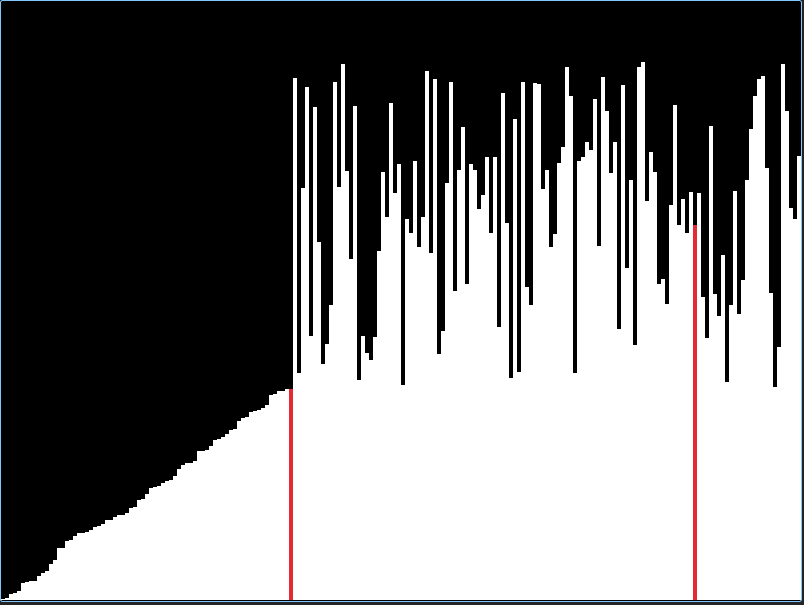
\includegraphics[width=0.85\linewidth]{sort-visi-screenshot.png}
  \caption{Sıralama görselleştiricisinin çalışırken alınmış ekran görüntüsü.}
  \label{fig:sort-visualizer}
\end{figure}

% ===========================================================================
\clearpage
\section*{Kaynakça}
\addcontentsline{toc}{section}{Kaynakça}
% ===========================================================================

\begin{itemize}
  \item BMT317 -- Algoritmalar ders sunumları, Doç. Dr. Adem Tekerek,
        Gazi Üniversitesi, 2026.
  \item cppreference.com, \emph{std::chrono::steady\_clock},
        \emph{std::vector} ve \emph{std::mt19937\_64}, erişim: 29.10.2026,
        \url{https://en.cppreference.com/w/}.
  \item Meson Build System Documentation,
        \url{https://mesonbuild.com/}.
  \item \emph{sortbench},
        \url{https://github.com/muratyalcin-ce/sortbench}.
  \item \emph{sort-visualizer},
        \url{https://github.com/muratyalcin-ce/sort-visualizer}.
\end{itemize}

\end{document}
